\subsubsection{UC 2.1 - Interazioni con la lista clienti}
\begin{figure}[H]
    \vspace{2em}
    \centering
    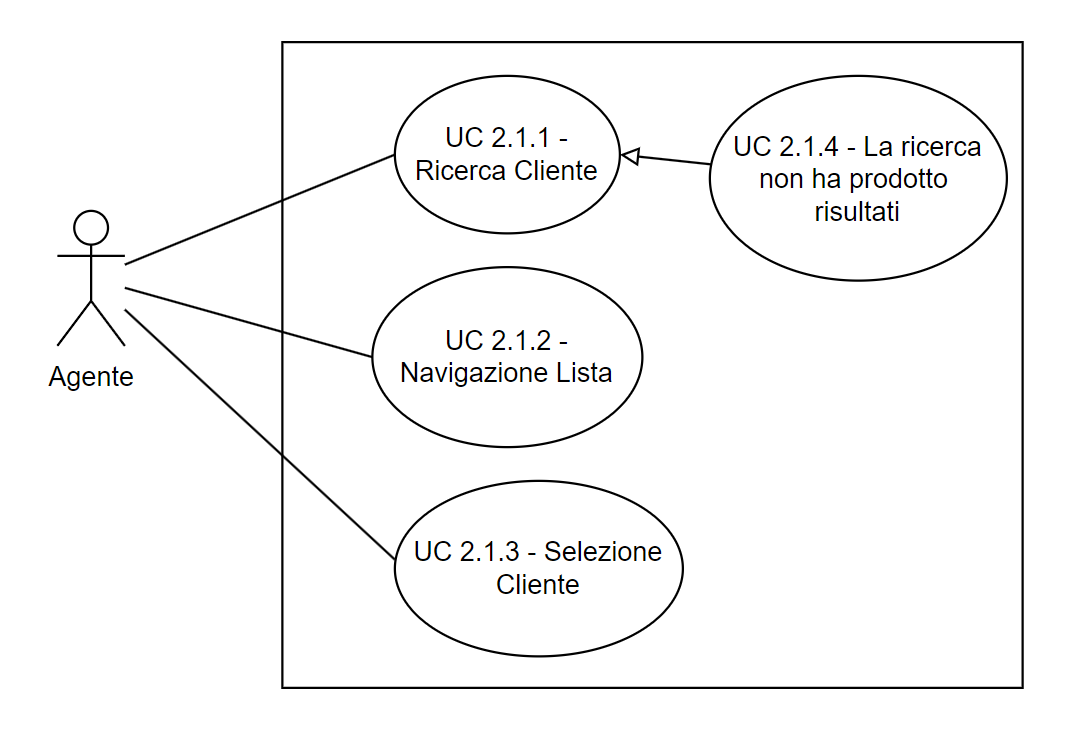
\includegraphics[width=0.75\columnwidth]{img/usecase/UC 2.1.png}
    \caption{\textit{Use Case} 2.1: Interazioni con la lista clienti}
    \label{fig:uc_2.1}
\end{figure}

\begin{usecase}{ 2.1.1}{Ricerca cliente}
    \usecaseactors{Agente.}
    \usecasedesc{L'agente ricerca un cliente specifico all'interno della lista clienti.}
    \usecasepre{
        \begin{itemize}
            \item L'utente si è autenticato con successo ed è stato riconosciuto come agente, quindi visualizza la 
                \texttt{Homepage Agenti};
            \item La lista clienti non è vuota.
    \end{itemize}}
    \usecasepost{L'agente visualizza il cliente ricercato.}
    \usecasescen{
        \begin{itemize}
            \item L'agente visualizza la \texttt{Homepage Agenti};
            \item L'agente visualizza la lista clienti;
            \item L'agente ricerca un cliente nella lista clienti;
            \item L'agente visualizza il cliente ricercato.
        \end{itemize}}
    \label{uc:uc_2.1.1}
\end{usecase}

\begin{usecase}{ 2.1.2}{Navigazione lista}
    \usecaseactors{Agente.}
    \usecasedesc{L'agente naviga la lista che contiene tutti i clienti dell'agente.}
    \usecasepre{
        \begin{itemize}
            \item L'utente si è autenticato con successo ed è stato riconosciuto come agente, quindi visualizza la 
                \texttt{Homepage Agenti};
            \item La lista clienti non è vuota.
    \end{itemize}}
    \usecasepost{L'agente è riuscito a navigare nella lista.}
    \usecasescen{
        \begin{itemize}
            \item L'agente visualizza la \texttt{Homepage Agenti};
            \item L'agente naviga la lista visualizzando i clienti contenuti.
        \end{itemize}}
    \label{uc:uc_2.1.2}
\end{usecase}

\begin{usecase}{ 2.1.3}{Selezione cliente}
    \usecaseactors{Agente.}
    \usecasedesc{L'agente seleziona un cliente per operare nell'\textit{app} come il cliente selezionato.}
    \usecasepre{
        \begin{itemize}
            \item L'utente si è autenticato con successo ed è stato riconosciuto come agente, quindi visualizza la 
                \texttt{Homepage Agenti};
            \item La lista clienti non è vuota.
    \end{itemize}}
    \usecasepost{L'agente viene spostato nella \texttt{Homepage} e può operare nell'\textit{app} come il cliente selezionato.}
    \usecasescen{
        \begin{itemize}
            \item L'agente visualizza la \texttt{Homepage Agenti};
            \item L'agente visualizza la lista clienti;
            \item L'agente seleziona un cliente;
            \item L'agente viene spostato nella \texttt{Homepage};
            \item L'agente può operare nell'\textit{app} come il cliente selezionato.
        \end{itemize}}
    \label{uc:uc_2.1.3}
\end{usecase}

\begin{usecase}{ 2.1.4}{La ricerca non ha prodotto risultati}
    \usecaseactors{Agente.}
    \usecasedesc{La ricerca di un cliente specifico all'interno della lista clienti non ha prodotto risultati.}
    \usecasepre{
        \begin{itemize}
            \item L'utente si è autenticato con successo ed è stato riconosciuto come agente, quindi visualizza la 
                \texttt{Homepage Agenti};
            \item La lista clienti non è vuota;
            \item L'agente ricerca un cliente.
    \end{itemize}}
    \usecasepost{L'agente visualizza il messaggio "nessun cliente trovato".}
    \usecasescen{
        \begin{itemize}
            \item L'agente visualizza la \texttt{Homepage Agenti};
            \item L'agente visualizza la lista clienti;
            \item L'agente ricerca un cliente nella lista clienti;
            \item La ricerca non produce risultati;
            \item L'agente visualizza il messaggio "nessun cliente trovato".
        \end{itemize}}
    \label{uc:uc_2.1.4}
\end{usecase}